\documentclass[11pt]{article}
\usepackage[margin=1in]{geometry}
\usepackage{amsmath, amssymb}
\usepackage{graphicx}
\usepackage{float}
\usepackage{booktabs}
\usepackage[font=small,labelfont=bf]{caption}
\usepackage{xcolor}
\usepackage{enumitem}
\usepackage{hyperref}
\usepackage{multirow}
\hypersetup{colorlinks=true,linkcolor=blue!60!black,urlcolor=blue!60!black}

\title{\Large\textbf{Hybrid GAD--Newton sweep}\\[4pt]
\normalsize 2026-05-04. Three step functions, two noise levels, five trust radii.\\[2pt]
\normalsize \emph{Standalone runner; separate from the main IRC test report.}}
\author{}
\date{}

\begin{document}
\maketitle
\thispagestyle{empty}

% =================================================================
\section*{What this sweep does}
% =================================================================

This document benchmarks three GAD--Newton hybrid step functions provided
as standalone step functions (separate from the rest of the project's level-4 NR
implementations, which had a documented negative result). Each step
function decides per-step whether to take a GAD step or an
eigenvector-following Newton step, and applies a trust-radius cap.

\textbf{Source files:}
\begin{itemize}[leftmargin=1.5em, itemsep=0.05em]
\item \texttt{src/gadplus/search/hybrid\_gad\_eigfollownewton.py}
  \\ \emph{plain hybrid:} \texttt{hybrid\_gad\_newton\_step\_from\_force(F, H, ...)}.
  No Eckart projection. Switch criterion: $\|F\|_2 < \mathtt{switch\_force}$
  triggers Newton; else GAD.
\item \texttt{src/gadplus/search/hybrid\_gad\_eigfollownewton\_eckart.py}
  \\ \emph{Eckart hybrid:} \texttt{projected\_hybrid\_gad\_newton\_step(F\_cart, H\_cart, coords, masses, ...)}.
  Eckart-projected mass-weighted internal coordinates. Switch toggle
  via \texttt{switch\_based\_on\_hessian\_eigval} (False: $\|F\|$ trigger;
  True: index-1 Hessian-clearance trigger).
\item \texttt{src/gadplus/search/hybrid\_gad\_damped\_eigfollownewton\_eckart.py}
  \\ \emph{Damped Eckart hybrid:} same interface as the Eckart variant
  with damped Newton step (mode $|\lambda_i|$ regularised by
  \texttt{min\_curvature}). Same switch toggle.
\end{itemize}

\textbf{Standalone runner:} \texttt{scripts/hybrid\_gad\_newton\_runner.py}
loops over T1x test split, per step calls HIP for $(E, F, H)$, runs the
the step function, applies the returned displacement (the step
function itself caps by trust\_radius internally), counts $n_{\text{neg}}$
on the Eckart-projected vibrational Hessian, terminates on
$n_{\text{neg}}{=}1 \wedge f_{\max}{<}0.01$. Up to 1000 steps.

\textbf{Sweep grid (50 cells):}
\begin{itemize}[leftmargin=1.5em, itemsep=0.05em]
\item \textbf{5 method-cells:} \{hybrid (no Eckart, force-switch),
  hybrid\_eckart switch=\{False, True\}, hybrid\_damped\_eckart switch=\{False, True\}\}
\item \textbf{2 noise levels:} 10 pm, 100 pm
\item \textbf{5 trust radii:} 0.005, 0.01, 0.02, 0.05, 0.10 (Å)
\end{itemize}

\textbf{Fixed:} $\mathtt{gad\_dt}{=}5\!\times\!10^{-3}$,
\texttt{switch\_force}${=}10^{-3}$, \texttt{min\_curvature}${=}10^{-6}$,
$n_{\text{samples}}{=}287$ test split, $n_{\text{steps}}{=}1000$, HIP
analytic Hessian every step.

\textbf{Reference baseline} (from the main report): vanilla GAD
dt=0.007 with 5000-step budget gets 89.2\% conv at 10pm and 72.8\% at
100pm. Vanilla GAD dt=0.005 (closer to this sweep's $dt$): 89.2\% / 71.8\%.

% =================================================================
\section{Headline grid}
% =================================================================

\begin{figure}[H]
\centering
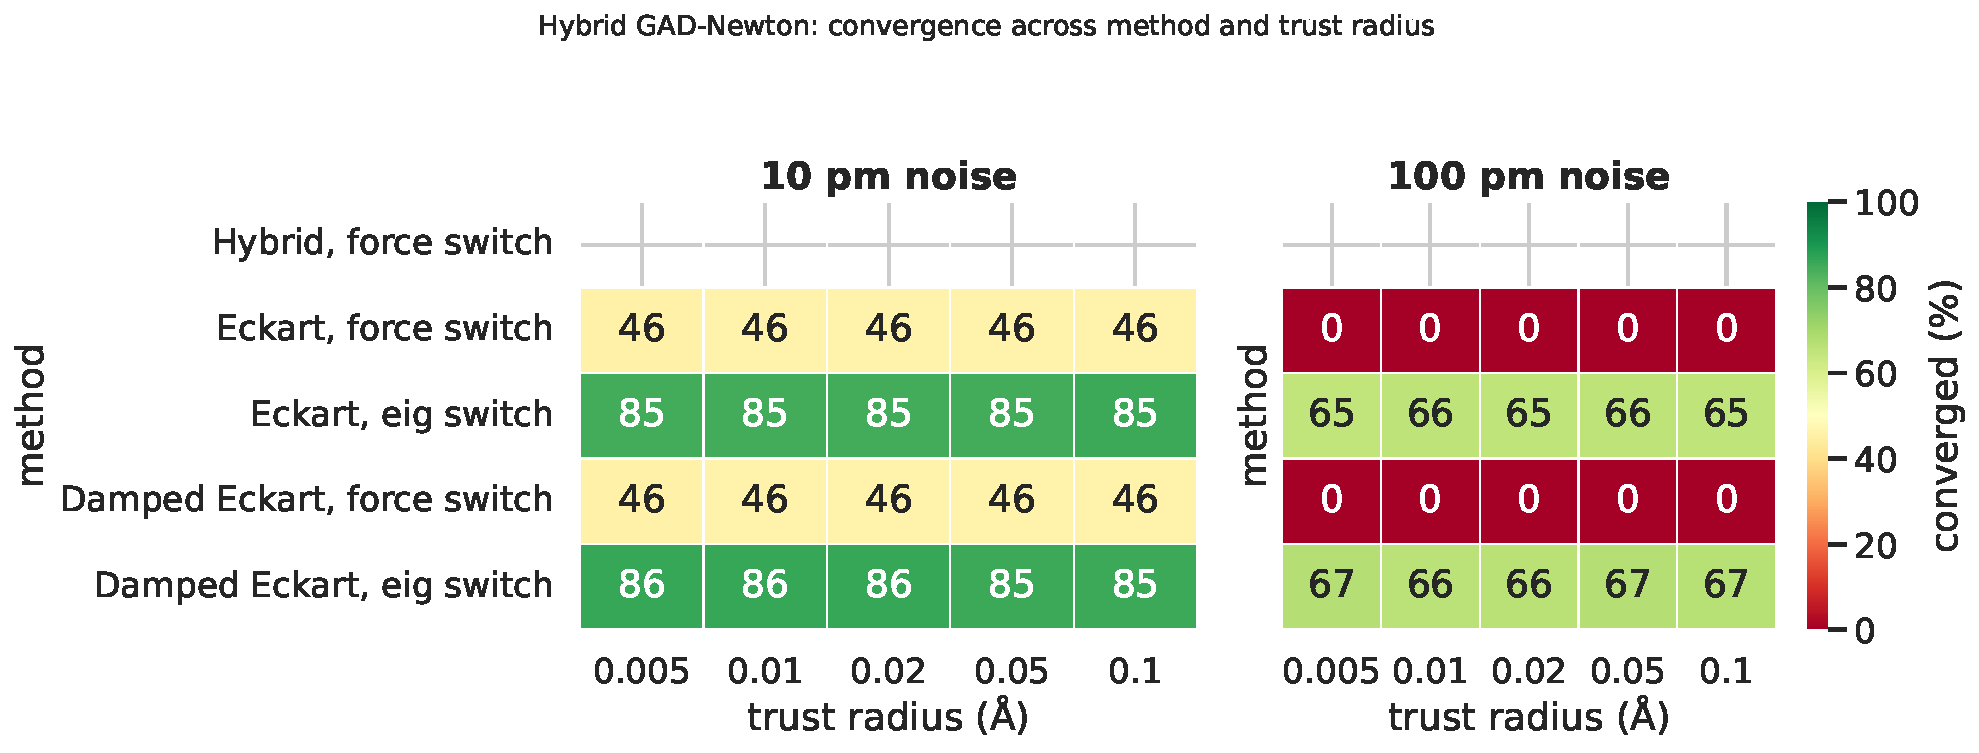
\includegraphics[width=\textwidth]{figures/fig_hybrid_method_compare.pdf}
\caption{Conv \% across the full 5-method × 5-trust-radius grid, per noise
level. Each cell is one of the 50 jobs ($n=287$ test samples,
$\le 1000$ steps). \textbf{Read the rows top-to-bottom for the method
spectrum; read the columns left-to-right for trust-radius effect.}
Reference: vanilla GAD dt=0.005 (closest non-hybrid baseline) gets
$\sim$89/72\% at the corresponding noise.}
\label{fig:hybrid-grid}
\end{figure}

\begin{figure}[H]
\centering
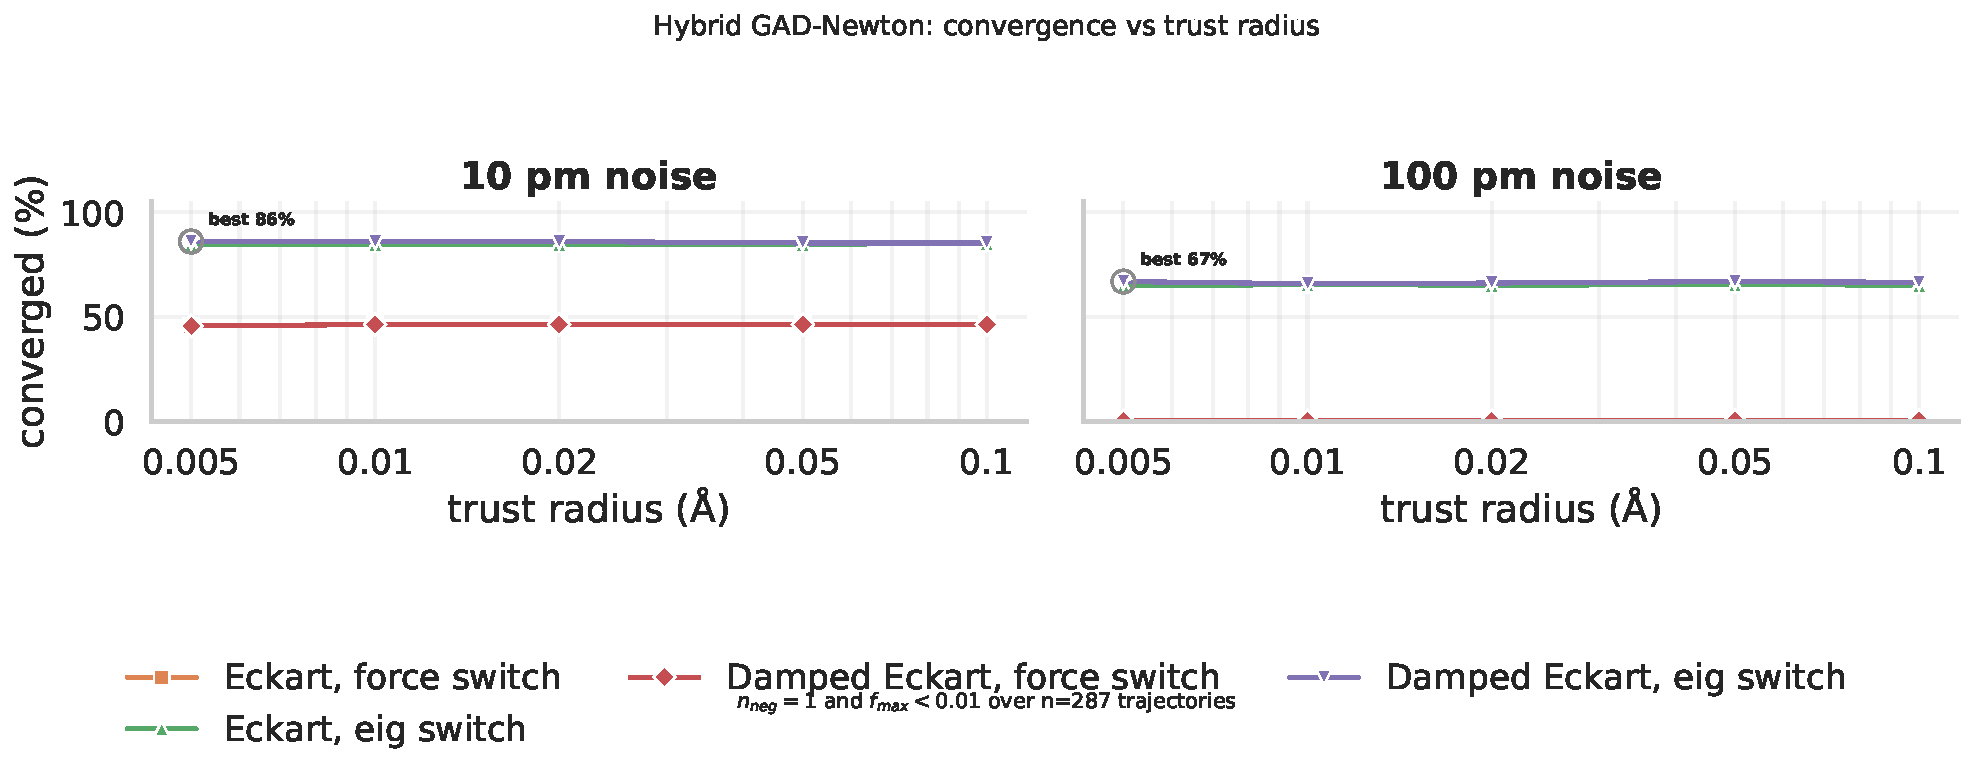
\includegraphics[width=\textwidth]{figures/fig_hybrid_conv_vs_tr.pdf}
\caption{Same data, line-form. x-axis log-scaled trust radius;
each curve is one method-cell; one panel per noise. Use this for
trust-radius scaling intuition: monotone, plateau, or non-monotone?}
\end{figure}

% =================================================================
\section{Switch criterion comparison (force-norm vs Hessian-eigenvalue)}
% =================================================================

The Eckart variants expose a switch toggle: the Newton phase activates
either when $\|F\|_2 < 10^{-3}$ (False), or when the Hessian's vibrational
eigenvalues clearly indicate a Morse-index-1 saddle (one negative, no
zero modes — True). The two should differ in \emph{when} they fire
during a trajectory: force-norm needs the trajectory to actually approach
$f_{\max} \ll 10^{-3}$ (which the main project's structural-plateau
analysis showed GAD essentially never does), whereas Hessian-clearance
fires as soon as the curvature signature is right, which can happen
earlier even with $f_{\max} \sim 10^{-2}$.

\begin{figure}[H]
\centering
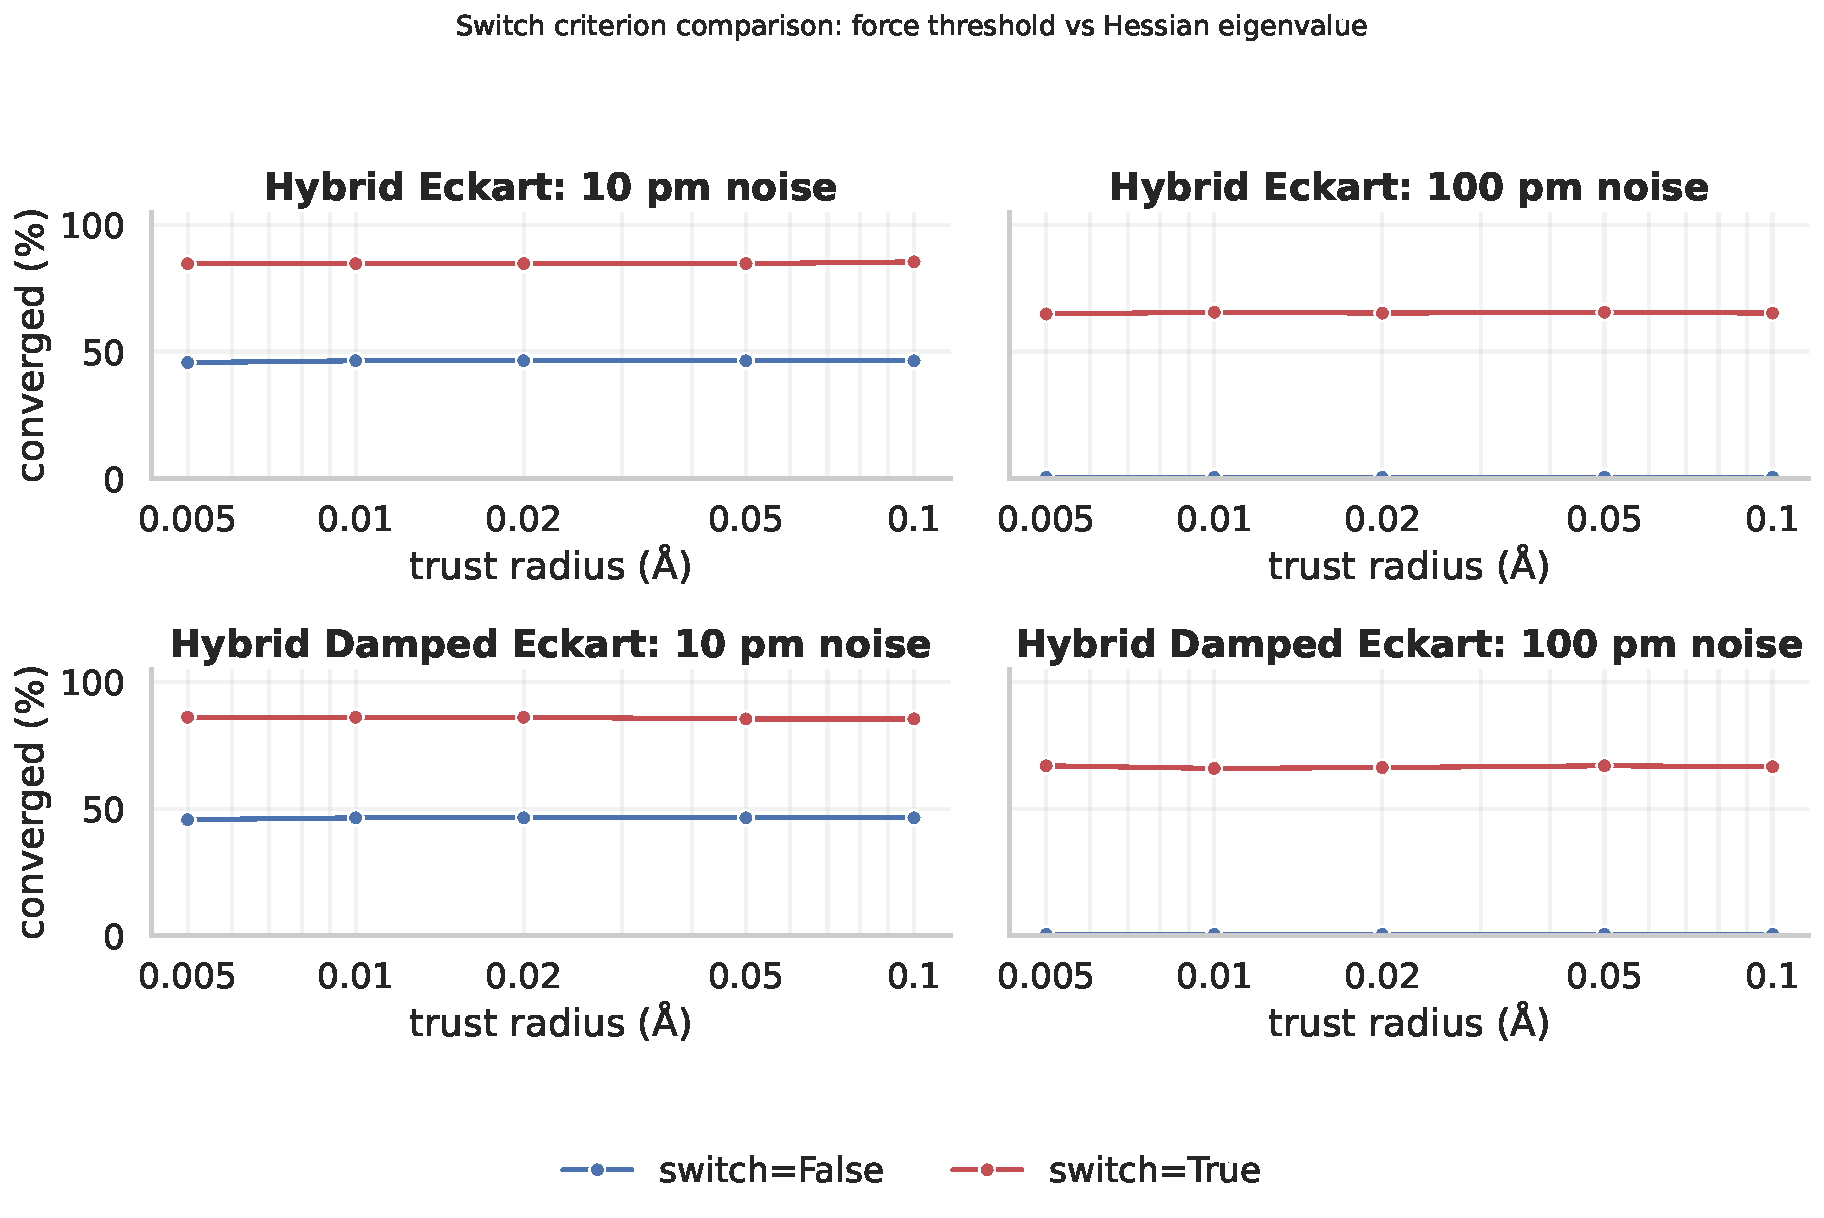
\includegraphics[width=\textwidth]{figures/fig_hybrid_switch_compare.pdf}
\caption{For both Eckart families (top: hybrid\_eckart; bottom:
hybrid\_damped\_eckart): switch=False vs switch=True curves.
\textbf{If switch=True activates Newton more often (which it should
given GAD's known fmax floor at $\sim$0.01), expect higher conv
or lower step counts at every trust radius.}}
\end{figure}

\begin{figure}[H]
\centering
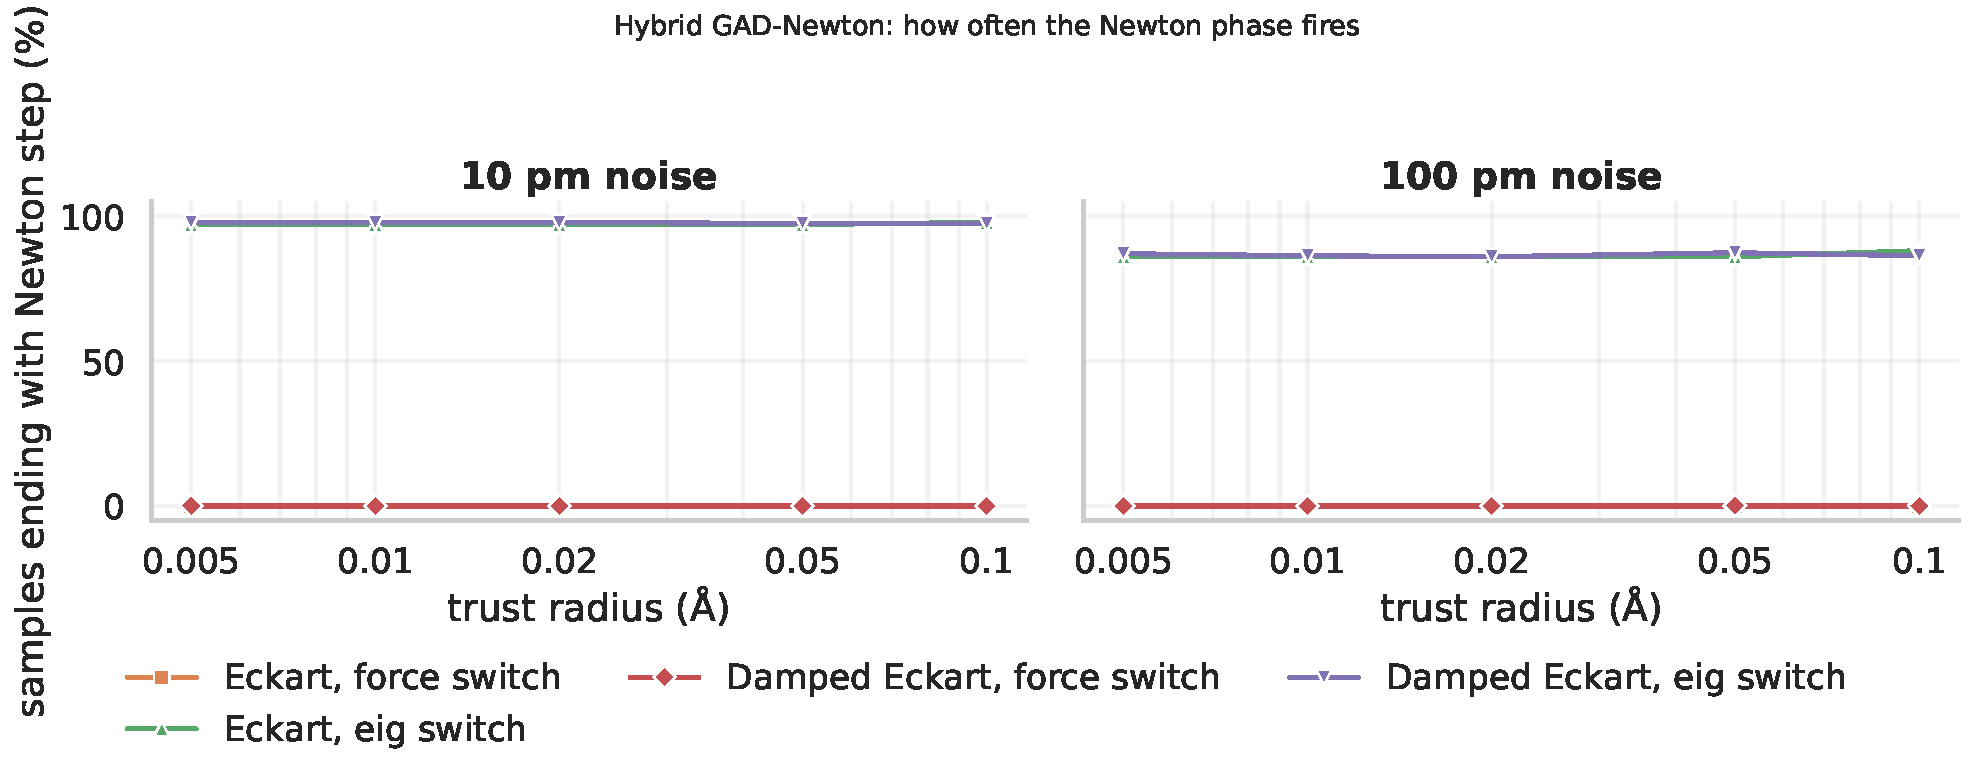
\includegraphics[width=\textwidth]{figures/fig_hybrid_step_phases.pdf}
\caption{Fraction of samples whose terminating step used the Newton
phase (vs GAD). With switch=False (force-norm trigger), this should be
near 0 because GAD plateaus around $f_{\max}\!\sim\!0.01$ and rarely
crosses $\|F\|<10^{-3}$. With switch=True, Newton should engage on every
sample that reaches index-1 saddle character — that's the design.}
\end{figure}

% =================================================================
\section{Compute (steps to converge)}
% =================================================================

\begin{figure}[H]
\centering
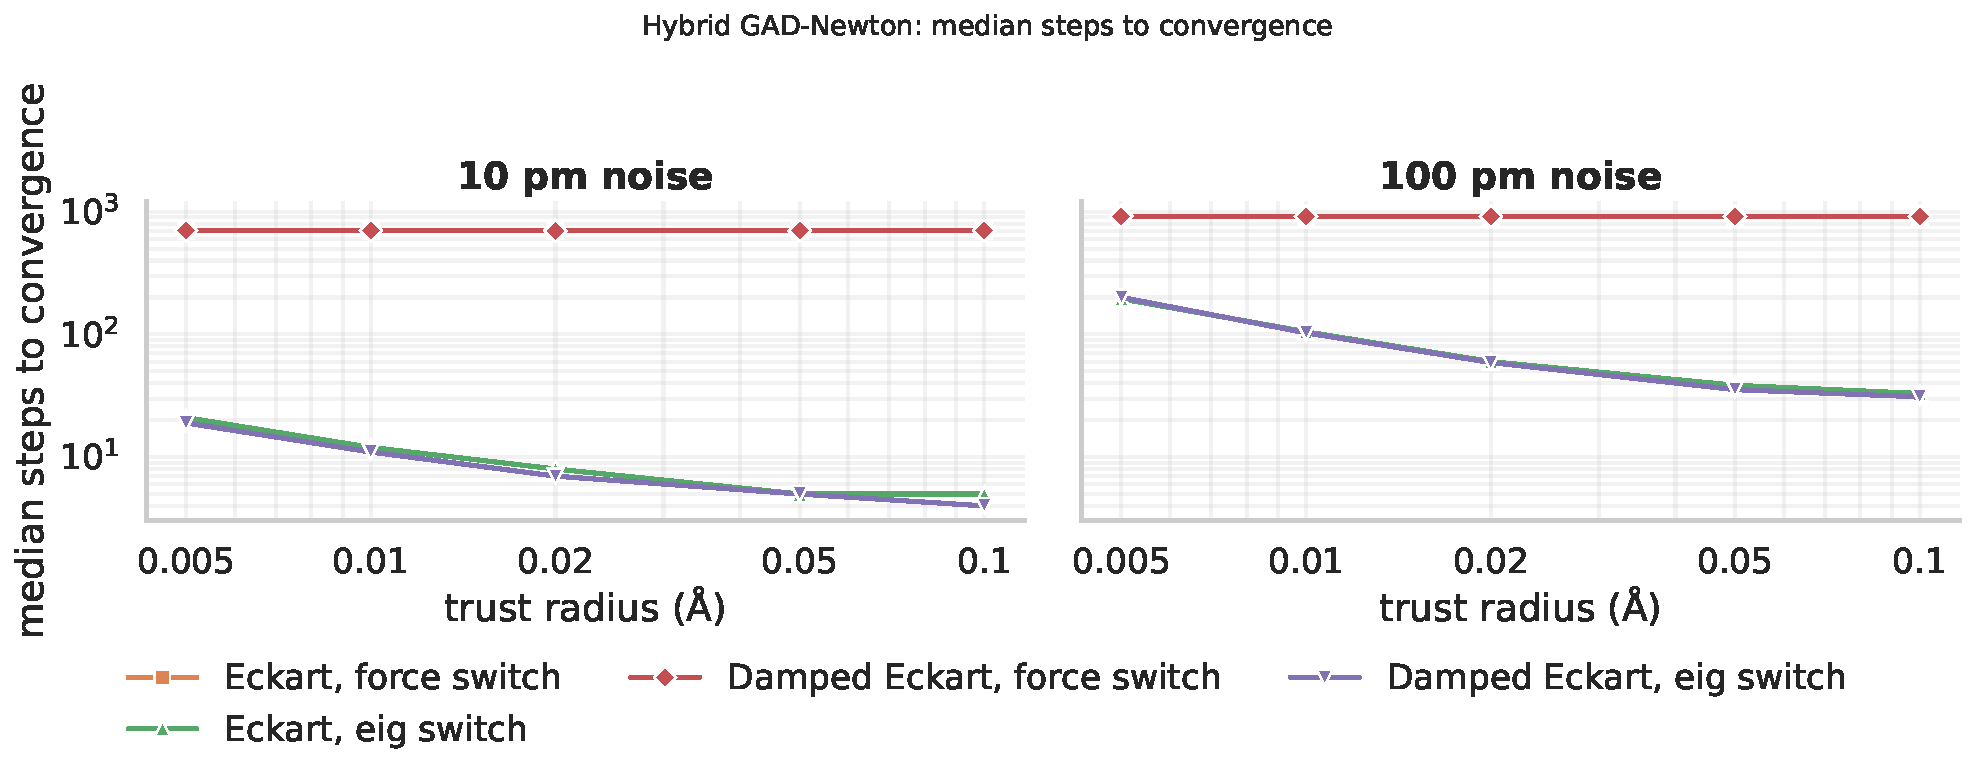
\includegraphics[width=\textwidth]{figures/fig_hybrid_steps_vs_tr.pdf}
\caption{Median steps to converge as a function of trust radius. Y-axis
log-scaled. \textbf{Smaller trust radius $\to$ more steps; the question
is whether the hybrid drops below vanilla GAD's median or not.}
At 100pm vanilla GAD takes $\sim$457 steps median (dt=0.005, 5k
budget); the hybrid sweep should be compared against that.}
\end{figure}

% =================================================================
\section{Tables}
% =================================================================

See \texttt{analysis\_2026\_04\_29/hybrid\_gad\_newton\_pivot.md} for the
machine-readable pivots.

\paragraph{Sources for every number:}
\begin{itemize}[leftmargin=1.5em, itemsep=0.05em]
\item Per-cell summary parquets:
  \texttt{runs/hybrid\_gad\_newton/<method\_tag>\_<noise>pm/summary\_*.parquet}
\item Aggregator:
  \texttt{analysis\_2026\_04\_29/hybrid\_gad\_newton\_summary.csv}
  (50 rows, one per cell).
\item Build script: \texttt{scripts/analyze\_hybrid\_gad\_newton.py}.
\item Standalone runner: \texttt{scripts/hybrid\_gad\_newton\_runner.py}.
\item SLURM array: \texttt{scripts/run\_hybrid\_gad\_newton.slurm} (job 60398168).
\item Step-function source files: see "What this sweep does" above.
\end{itemize}

\end{document}
